\documentclass[11pt,a4paper]{article}

\usepackage{graphicx}
\title{Designing of Power Management Circuitry for R-PI}
\author{e-Yantra Team}
\date{\today}

\begin{document}
	\maketitle
	\newpage
	\tableofcontents
	\newpage
	
\section{Objective}
The objective is to design a Power Management assembly which can perform the following operations:
		\begin{itemize}
			\item Battery voltage monitoring and Smart battery charging
			\item Regulated supply for on-board payload
			\item On board Switching from a battery source to an Auxiliary Power Source
		\end{itemize} 
	\section{Prerequisites}
	One should have:
	\begin{itemize}
		\item Some knowledge about the Current and Voltage Laws governing the design of a circuit.
		\item Some basic information regarding Power requirements of the system. Like current and  Voltage ratings of payload attached to the R-pi.
        \item the concept of the Regulators should be known.
	\end{itemize}

	\section{Hardware Requirement}
	\begin{enumerate}
		\item NiMH battery and Power adapter as an auxiliary source unit.
		\item Voltage Regulator ICs Ua-7805, LMS-1585
		\item Dot or Bargraph Display driver IC LMS-3914 
		\item Resistors, Capacitors and Connecting wires
	\end{enumerate}
	
	\section{Software Requirement}
	\begin{enumerate}
		\item OSCAD.
		\item Fritzing.
		%		\item Dot or Bargraph Display driver IC LMS-3914 
		%		\item Connecting wires
	\end{enumerate}	
	
	
	
	\section{Theory and Description}
	\subsection{Voltage Supply Unit}
	The battery used in this project is a rechargeable 9.6V, 2.1 Ah Nickel Metal Hydride battery which can power the R-pi assembly for approximately 2 hours. The output of this battery is used to drive R-pi and Payload attached to it. the payload are Sensors, Motors, port expander IC' s  or ADC IC' s and display units like LCD. They generally depend on the type of application. These components use different supplies and hence the output from the battery are dropped and regulated to appropriate level using the regulators to obtain the desired output Voltage Level. In this section regulators used are discussed in brief.    	
	
	\subsection{uA-7805}    
	This series of fixed-voltage Regulators are designed for a wide range applications. These applications include on-card regulation for elimination of noise and distribution.These regulators can deliver up to 1.5 A of output current.
	
	    \begin{figure}[h!]
	    	
	    	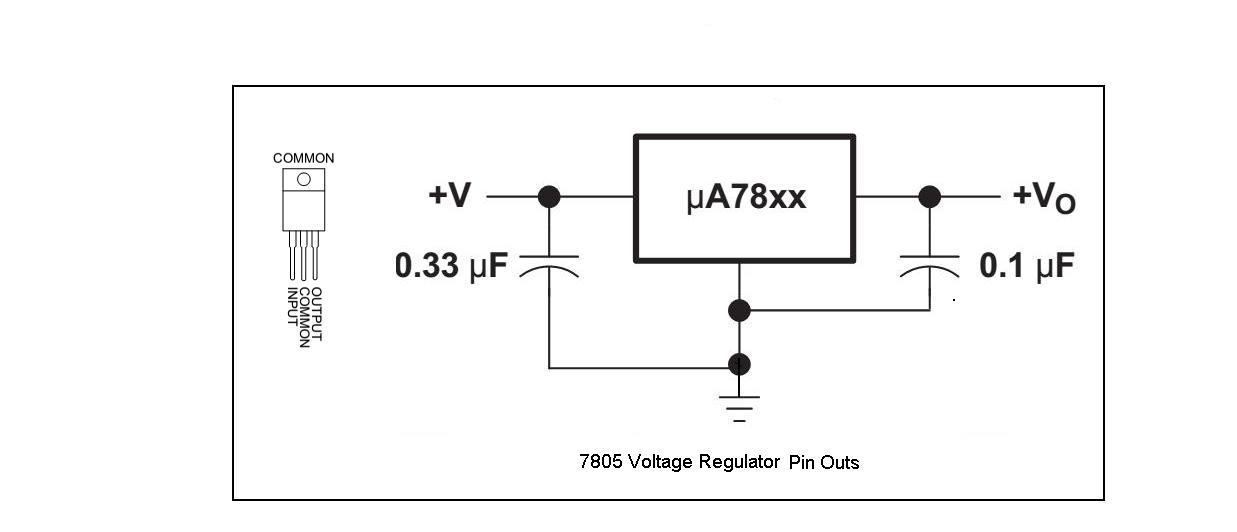
\includegraphics[scale=0.4]{7805.jpg}
%	    	\left. 
			\caption{7805 Voltage Regulator}
	    \end{figure}
	
	Some of the features of this regulator are listed as follows
	\begin{itemize}
		\item 3-Terminal Regulators.
		\item Output Current up to 1.5 A.
		\item Internal Thermal-Overload Protection.
		\item High Power-Dissipation Capability.
		\item Internal Short-Circuit Current Limiting ability.
		
	\end{itemize} 


	\subsection{LMS-1585a Variable Voltage Regulator} 
	LMS-1585 voltage Regalators are used to provide 3.3V Supply to the R-pi. The low dropout voltage (1.2V) and
	fast transient response make them an excellent solution for low voltage microprocessor applications.
	
	 The LMS1585A/87 series are available in KTT (TO-263) and NDE (TO-220) packages.
	 \begin{figure}[h!]
	 	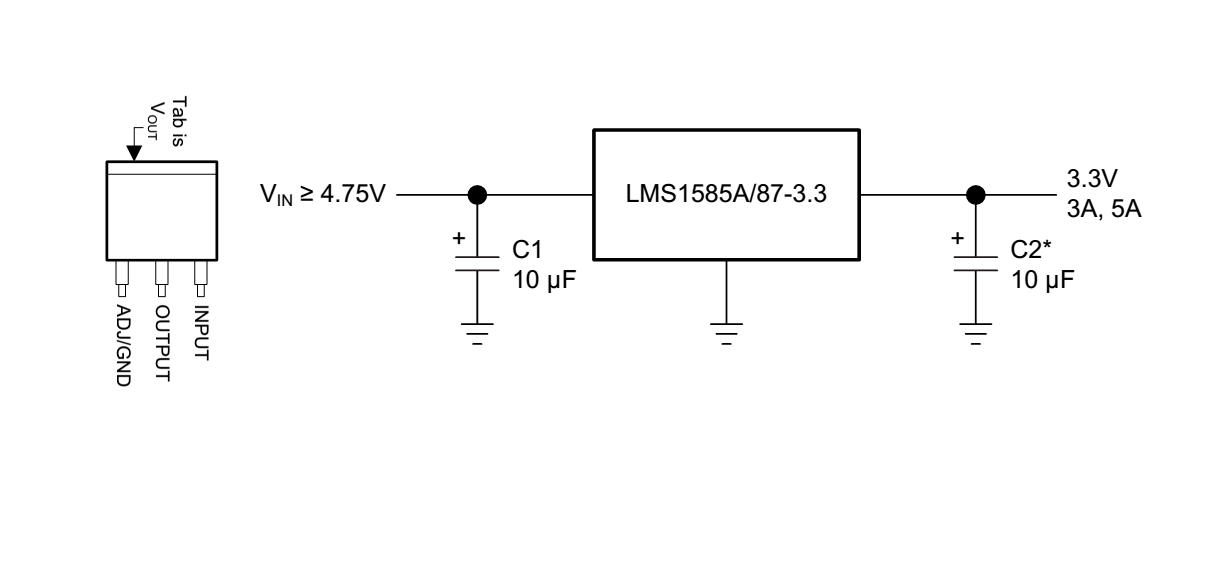
\includegraphics[scale=0.49]{1585.jpg}
	 				\caption{LMS-1585 Voltage Regulator}
%	 	\centering
	 \end{figure}
	
	\begin{itemize}
		\item The LMS1585A is a low dropout positive regulators with output load current of 3A.
		\item they offer low dropout voltage (1.2V) and hence fast transient respons
		\item they are available in adjustable versions, which can set the output voltage with only two external resistors.
		\item They have built in Current Limiting and Thermal Protection Circuitry. 
		\item Maximum Input to Output Voltage (VIN to GND) 13V and Power Dissipation is Internally Limited
	\end{itemize}
	
	
	\subsection{Basic Adjustment for Regulator}
	The adjustable version develops at 1.25V reference voltage, (VREF), between the output and the adjust terminal. As shown in Figure 3, this voltage is applied across resistor R1 to generate a constant current I1. This constant current then flows through R2. The resulting voltage drop across R2 adds to the reference voltage to sets the desired output voltage.
	The current IADJ from the adjustment terminal introduces an output error. But since it is small (120μA max), it becomes negligible when R1 is in the 100Ω range. For fixed voltage devices, R1 and R2 are integrated inside the devices.
	\begin{figure}[h!]
	
		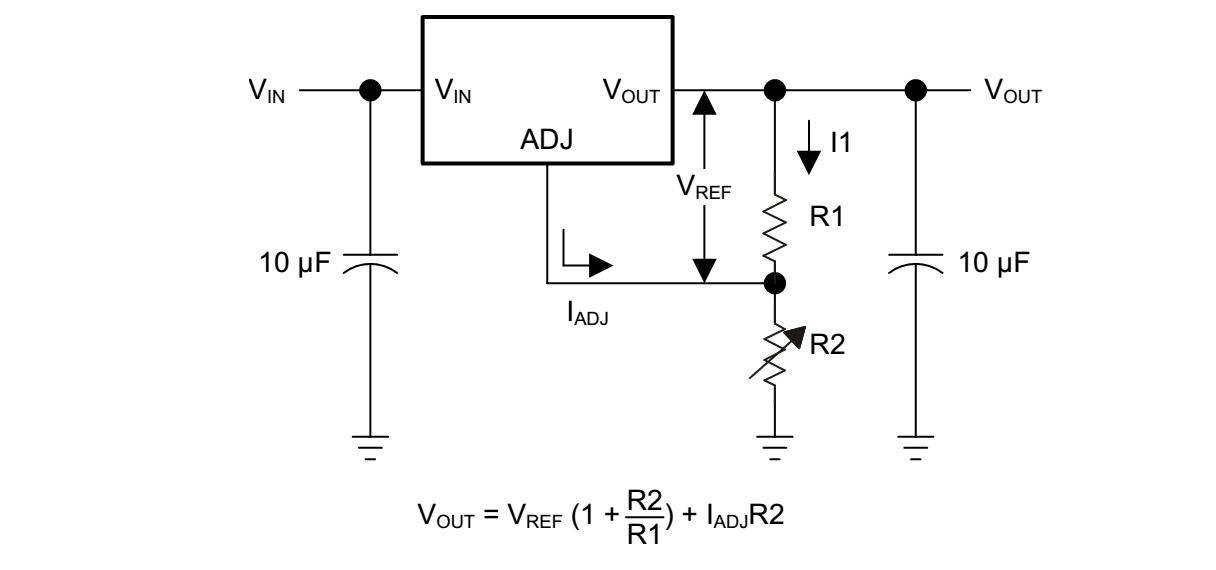
\includegraphics[scale=0.43]{adj1585.jpg}
			\caption{Basic Adjustable Regulator}
		%\centering
	\end{figure}
	
	
	Here we have set the value of resistance R1=1.2K $\Omega$ and for Output Voltage of 3.3V and We got R2=1.96K $\Omega$ . It is set according to Formula shown in Figure 3.
	
		\section{Battery Monitoring}
	The whole Raspberry-Pi assembly and payload are powered by 9.6V rechargeable
	 Nickel Metal Hydride battery pack. The battery voltage can vary between 12V (fully charged) to 8V (discharged). Battery pack should not be discharged below 8V (1V per cell) for extended battery life.
	 
%	 \ref{}
		
	\paragraph{Note}: When the battery reaches full charge, the energy being supplied to the battery is no longer being consumed in the charge reaction, and must be dissipated as heat within the cell. This results in a very sharp increase in both cell temperature and internal pressure.The cell contains a pressure-activated vent which should open if the pressure gets too great,  if charging is continued Further, the Ni-MH cells release hydrogen gas, which will burn violently if ignited.
	
	To prevent Overcharging and fully discharging of the battery a  circuitry is required to correctly indicate the user about the voltage levels in the battery for this purpose we have used Texas Instrument manufactured LM3914 dot or bar display driver IC.In this Circuit two LED's are used to indicate full charge indication(12v) and discharge voltage Level(8v).
	
	
	\subsection{LMS-3914}
	The LM3914 is a monolithic integrated circuit that senses analog voltage levels and drives 10 LEDs,	providing a linear analog display A single pin changes the display from a moving dot to a bargraph. Current drive to the LEDs is regulated and programmable, eliminating the need for resistors.This feature is one that allows operation of the whole system from less than 3V.



Some of the features of this IC are as follows	
\begin{itemize}
\item Drives LEDs, LCDs or Vacuum Fluorescents.
\item this IC can be operated in Bar or Dot Display Mode Externally Selectable by user.
\item Internal Voltage Reference from 1.2V to 12V.
\item The Internal 10-step Divider is Floating and can be Referenced to a Wide Range of voltages.
\item LED Driver Outputs are Current Regulated, open collector ed.
\end{itemize}

	\subsection{Use of LM3914 to Monitor 12V}

	\begin{figure}[h!]
		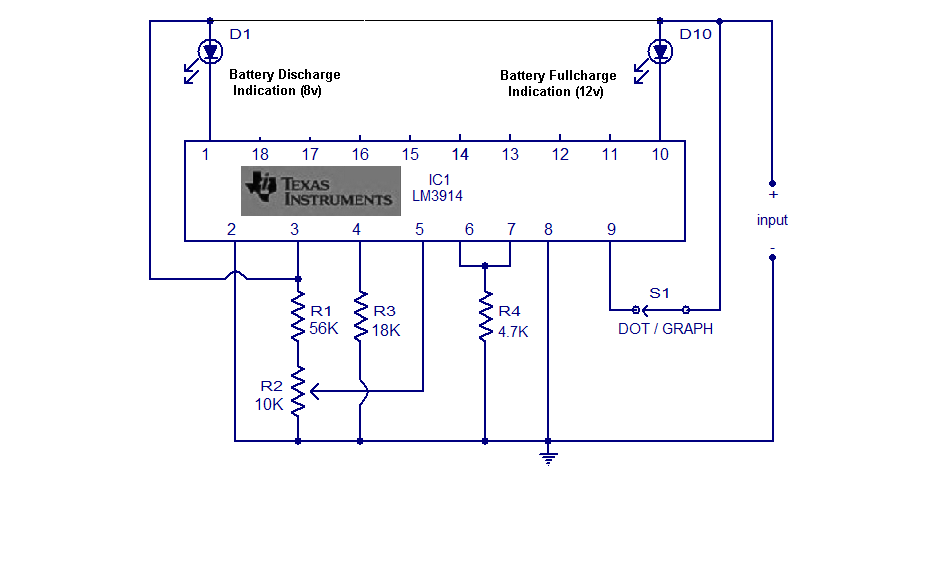
\includegraphics[scale=0.5]{3914.jpg}
		\centering
	\end{figure}

\newpage
	\begin{figure}[h!]
		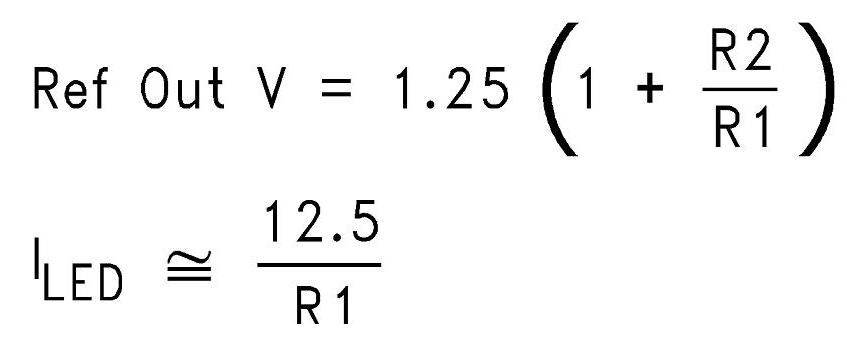
\includegraphics[scale=0.3]{eq.jpg}
		\centering	
		\caption{LMS-3914 Dot or Bargraph Display Driver}
	\end{figure}
	
\begin{itemize}
\item Switch S1 can be used to select between dot mode and bar graph mode. When S1 is
closed, pin9 of the IC gets connected to the positive supply and bar graph mode gets enabled.
\item Here the switch is opened to operate the device in dot mode.
    \item Resistor R4 connected between pins 6,7 and ground controls the brightness
    of the LEDs.Increasing the value of resistance decreases the brightness of the LED's.
    
    \item  Resistors R1 and POT R2 forms a voltage divider network and the POT R2 can be used for calibration.
    
    \item The upper Limit is calibrated using R2. First the required upper Voltage is set using an Regulated Power Supply unit and by adjusting the pot at R2  the upper Limit is set.
    \item For adjusting the lower limit, Replace the R1 resistor(s) with a 100K potentiometer (as shown above), connect the desired lower limit voltage to the monitor and adjust the 100K potentiometer until the first red LED just turns on.
    \item Now replace the Pot by the resistance obtained during calibration.
\end{itemize}

\textbf{Note: The circuit Can be powered up by using an auxiliary Source - a 12v adapter . For this change the Position of Switch at Position-2. The Adapter Connected at Auxiliary Power Slot Connects to the Circuit Providing the required supply Voltages.This is indicated in Figure 5 and Figure 6}

%	\subsection{Use of LM3914 to Monitor 12V}
\newpage
	\begin{figure}[h!]
		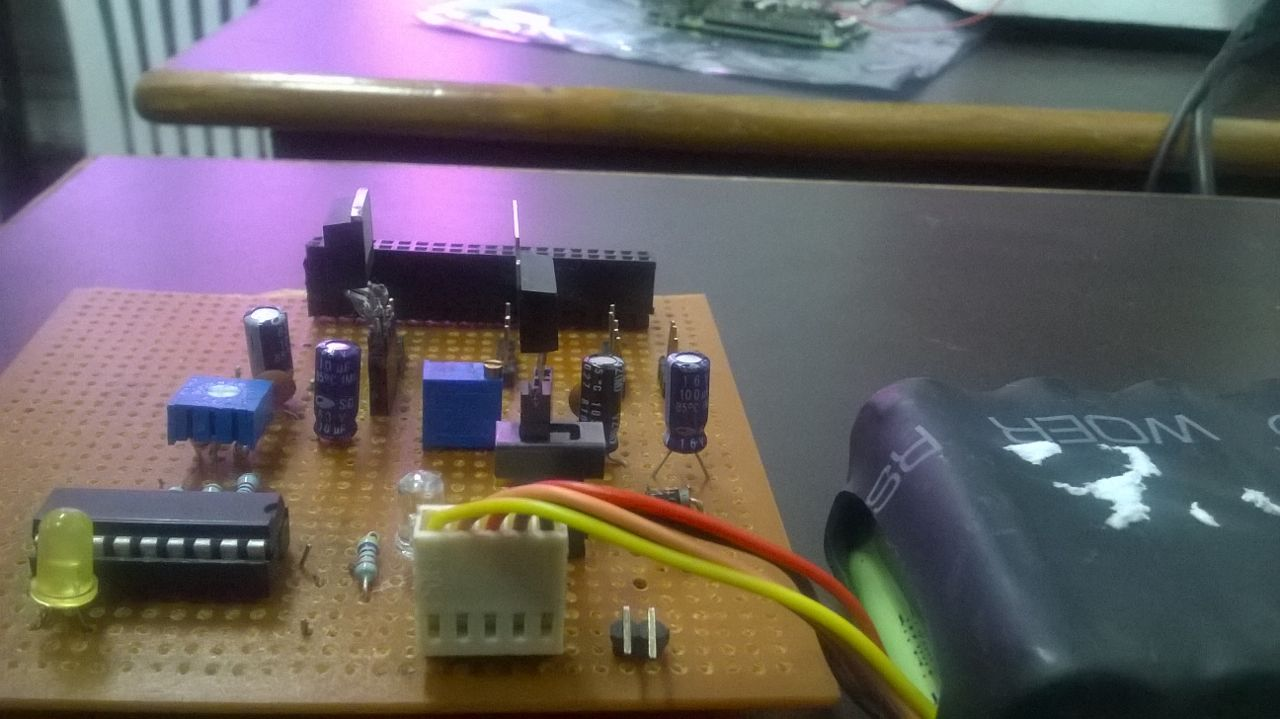
\includegraphics[scale=0.3]{im1.jpg}
		\centering
		\caption{Powering Up of Cicuit Using Battery}
		\textbf{Note: Here Switch is at Position-1.}
		
		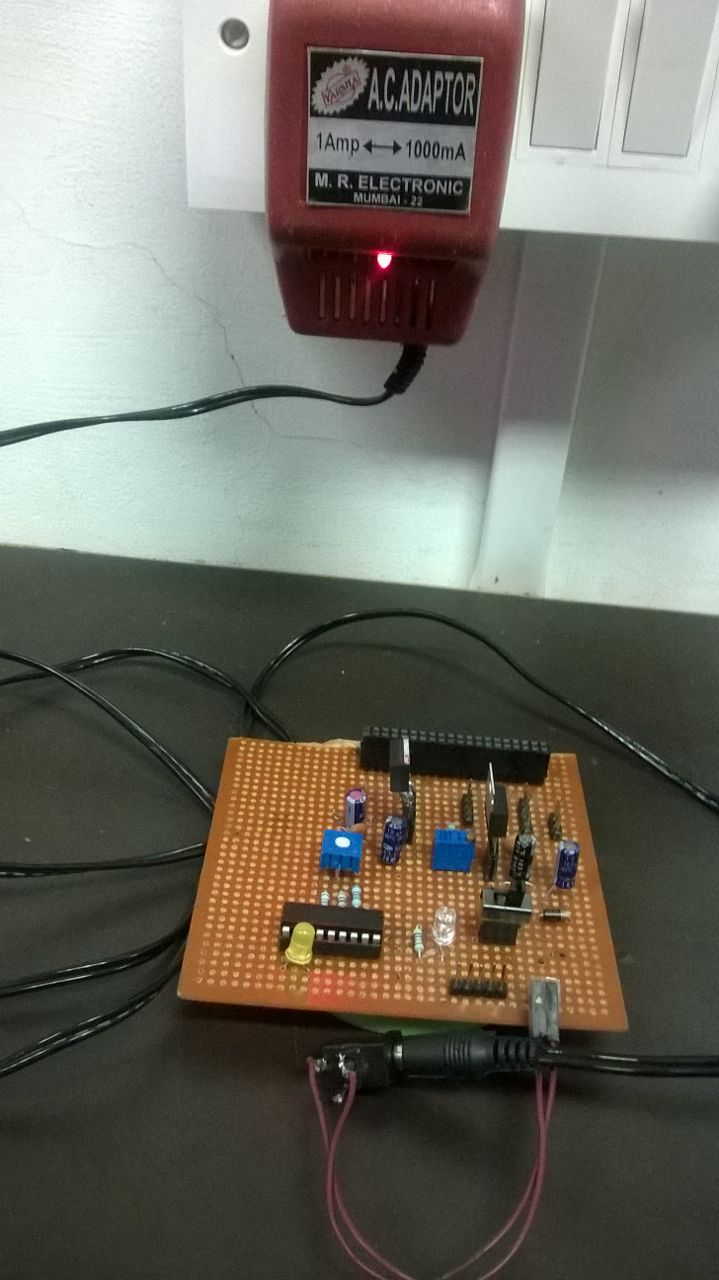
\includegraphics[scale=0.3]{im2.jpg}
		\centering	
		\caption{Powering Up of Cicuit Using Adapter}
			\textbf{Note: Here Switch is at Position-2.}
	\end{figure}

\newpage
	\section{PCB Designing using Oscad}
	\subsection{Schematic Design}
	The Schematic Design is shown in figure 6.
		\begin{figure}[h!]
			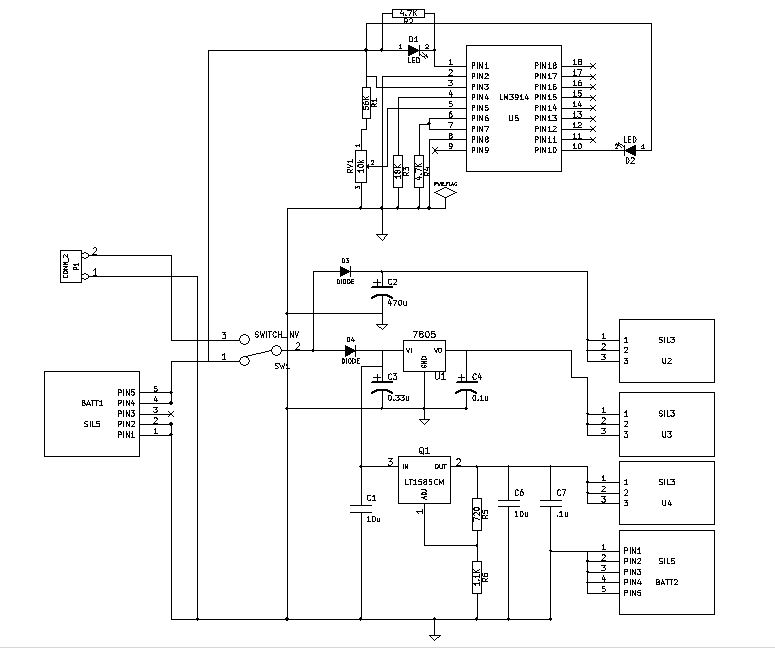
\includegraphics[scale=0.5]{sch.jpg}
			\centering

			\caption{PCB Schematic of the Power Management Circuit}
		\end{figure}
	
	
		\subsection{PCB Layout}
			The PCB Layout is shown in figure 7.
		\begin{figure}[h!]
			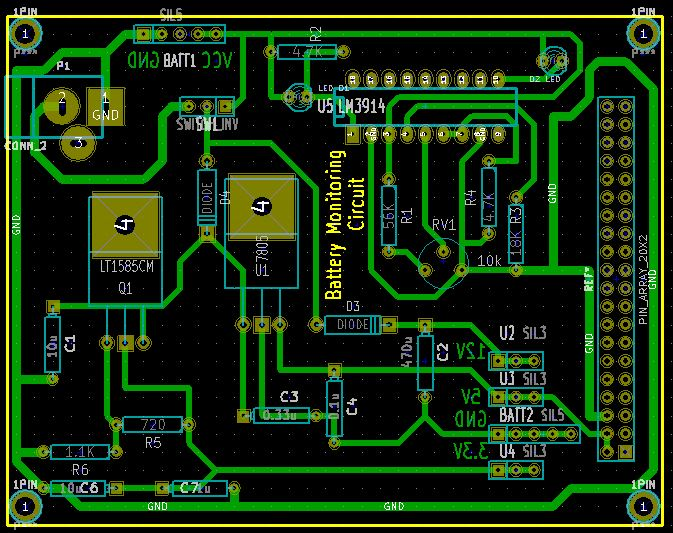
\includegraphics[scale=0.5]{pcb.jpg}
			\centering
			
			\caption{PCB Layout of the Power Management Circuit}
		\end{figure}
		
		
			\newpage
			\section{References}
			\begin{enumerate}
				\item Firebird-V Hardware Manual
				\item uA7805, LMS1585 and LM3914 Datasheets. 
				\item http://batteryuniversity.com/learn/article/sharing\_battery\_knowledge
				\item http://www.ti.com/lit/an/snva557/snva557.pdf	
			\end{enumerate}
		
		
\end{document}



